\documentclass[11pt,a4paper]{article}
\usepackage[utf8]{inputenc}
\usepackage[spanish]{babel}
\usepackage{amsmath}
\usepackage{amsfonts}
\usepackage{amssymb}
\usepackage{graphicx}
\usepackage{booktabs}
\usepackage{siunitx}
\usepackage{caption}
\usepackage{subcaption}
\usepackage{geometry}
\geometry{margin=2.5cm}

\sisetup{
  separate-uncertainty = true,
  per-mode = symbol
}

% Datos de la práctica
\def\numeroPractica{10}
\def\tituloPractica{Característica resistencia-temperatura de un termistor}

\title{Práctica \numeroPractica: \tituloPractica}
\author{Andrés}
\date{\today}

\begin{document}

\maketitle

\begin{abstract}
En esta práctica se estudia la dependencia de la resistencia eléctrica de un termistor con la temperatura absoluta. A partir de medidas experimentales, se verifica el modelo exponencial $R = A e^{B/T}$. Los parámetros característicos del termistor se obtienen mediante dos aproximaciones: un cálculo analítico a partir de dos puntos de referencia y un ajuste no lineal por regresión de distancia ortogonal (ODR) considerando incertidumbres en ambas variables. El ajuste ODR proporciona los valores $A = (1.59 \pm 0.08) \times 10^{-5} \text{ k}\Omega$ y $B = 3973 \pm 14 \text{ K}$, con un excelente coeficiente de bondad de ajuste, confirmando la validez del modelo teórico asumido.
\end{abstract}

\section{Introducción y Objetivos}
% [HUMAN AUTHOR: INTRODUCCIÓN AQUÍ]
El objetivo de esta práctica es determinar la relación experimental entre la resistencia eléctrica de un termistor y su temperatura absoluta, ajustando los datos a un modelo exponencial de la forma $R = A e^{B/T}$.

\section{Resultados}

\subsection{Cálculo analítico a partir de dos puntos}
Se han seleccionado dos puntos de referencia para realizar un cálculo preliminar de los parámetros $A$ y $B$:
\begin{itemize}
    \item $T_1 = \qty{353.15 \pm 0.10}{K}$, $R_1 = \qty{1.25 \pm 0.22}{k\Omega}$
    \item $T_2 = \qty{273.25 \pm 0.10}{K}$, $R_2 = \qty{31.50 \pm 0.58}{k\Omega}$
\end{itemize}

A partir de la solución analítica del sistema de ecuaciones:
\begin{equation}
    B = \ln\left(\frac{R_1}{R_2}\right) \frac{T_1 T_2}{T_2 - T_1} \quad ; \quad A = R_1 e^{-B/T_1}
\end{equation}
Se han obtenido los siguientes valores:
\begin{itemize}
    \item $A = \qty{2.0 \pm 1.6e-5}{k\Omega}$
    \item $B = \qty{3890 \pm 210}{K}$
\end{itemize}
Este método proporciona una estimación inicial de los parámetros, pese a que es ampliamente suscepctible a errores, debido a que
solo se toman dos medidas, este método proporciona una buena estimación de parámetros para así obtener un buen punto de partida para el algoritmo
en la siguiente sección, el cual es más robusto al considerar todas las medidas experimentales.

\subsection{Representación gráfica y Ajuste ODR}
Se ha representado el logaritmo de la resistencia en función de la inversa de la temperatura absoluta ($1/T$), lo cual debería mostrar una tendencia lineal según la ecuación $\ln(R) = \ln(A) + B/T$.

\begin{figure}[ht!]
    \centering
    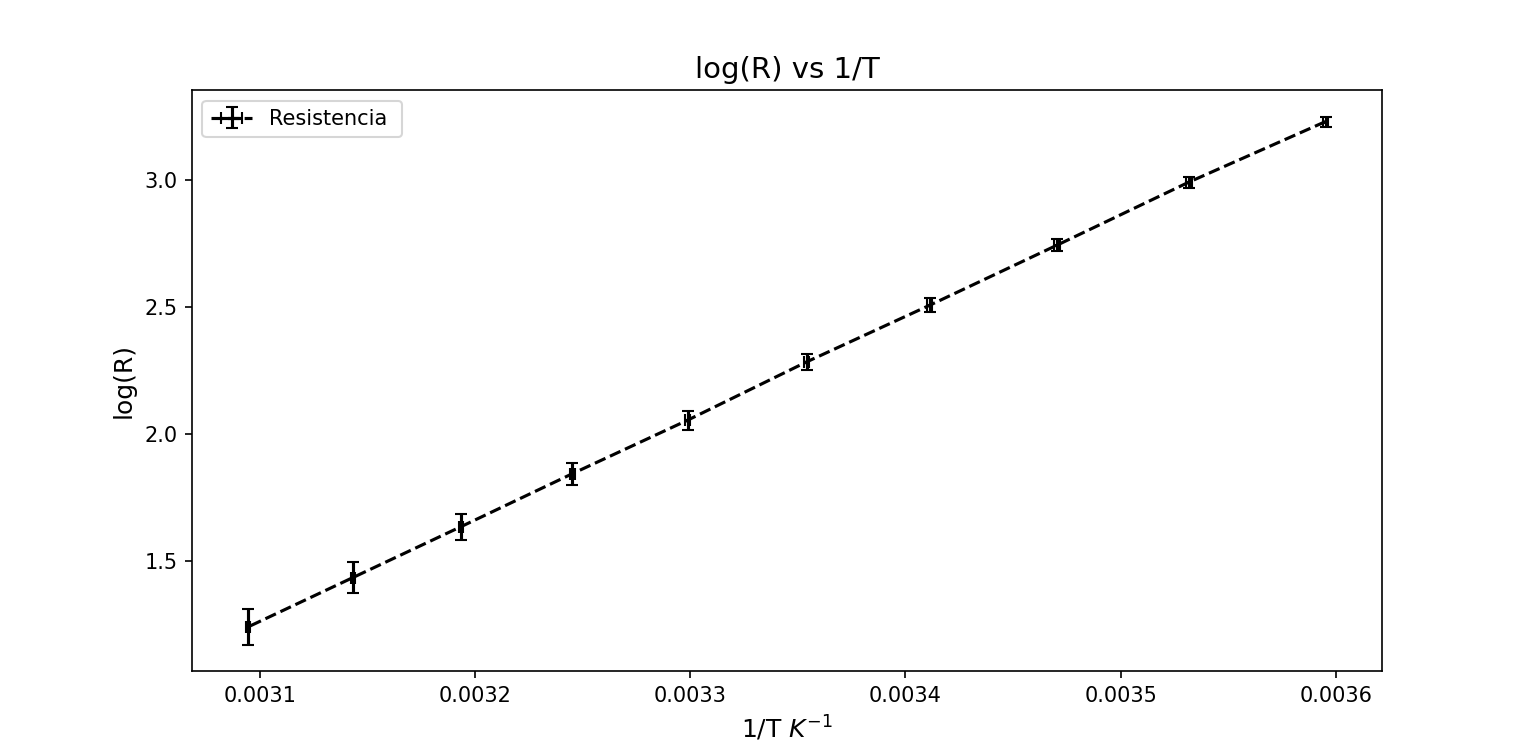
\includegraphics[width=0.8\textwidth]{logvst.png}
    \caption{Representación de $\ln(R)$ frente a $1/T$ ($K^{-1}$).}
    \label{fig:logvst}
\end{figure}

Posteriormente, se ha realizado un ajuste no lineal mediante el método de Ortogonal Distance Regression (ODR) sobre la relación $R = A e^{B/T}$, considerando errores en ambas variables. Los parámetros obtenidos del ajuste son:
\begin{itemize}
    \item $A = \qty{1.59 \pm 0.08e-5}{k\Omega}$
    \item $B = \qty{3973 \pm 14}{K}$
    \item Coeficiente de determinación $R^2 = 0.999876$
\end{itemize}


Dado que $R^2 \approx 1$, se puede concluir que existe una correlación entre ambas variables, sin embargo, no podemos concluir que esta sea la correcta,
ya que es posible que haya factores externos que no modifiquen la correlación, pero sí modifiquen la relación entre ambas variables, por lo que es importante analizar los resultados con cautela.
Por ejemplo, una de las posibles limitaciones del modelo teórico es que no considera temperaturas extremas, muy bajas o muy altas, que podrían alterar la estructura misma del material,
lo cual podría modificar esta relación entre resistencia y temperatura, por ende es de vital importancia considerar que los resultados obtenidos en esta práctica
solamente son válidos para el rango de temperaturas estudiado, y no se pueden extrapolar a temperaturas extremas sin realizar un análisis más detallado.
\subsection{Medición de temperatura}
Para contrastar nuestros hallazgos, sumergiremos el termistor en un baño de agua a temperatura ambiente, y mediremos su resistencia, para así comparar el valor medido con el valor predicho por el modelo, y así verificar la validez del mismo.
usaremos la siguiente ecuación para calcular la temperatura del agua a partir de la resistencia medida:
\begin{equation}
    T = \frac{B}{\ln(R/A)}
\end{equation}
Una vez realizado el cálculo, se ha obtenido una temperatura de \qty{21.4 \pm 2.3}{\degreeCelsius}, lo cual corresponde a una temperatura de \qty{22.35 \pm 1.5}{\degreeCelsius}, lo cual es razonable para la temperatura ambiente del laboratorio.

\section{Conclusiones}
% [HUMAN AUTHOR: ESCRIBE LAS CONCLUSIONES AQUÍ]
% Resume los aspectos más relevantes y reflexiona sobre los resultados obtenidos.
Esto es una geminada chema, pon tu algo
\appendix
\section{Anexos}

\subsection{Tablas de datos}
En la Tabla~\ref{tab:datos_experimentales} GEMINADAAA REVISAR se muestran los valores medidos de temperatura y resistencia con sus respectivas incertidumbres.

\begin{table}[ht!]
    \centering
    \begin{tabular}{S[table-format=2.1] S[table-format=3.2] S[table-format=1.2] S[table-format=2.2] S[table-format=1.3]}
    \toprule
    {Temp. (\unit{\degreeCelsius})} & {Temp. (\unit{K})} & {$u_T$ (\unit{K})} & {Resistencia (\unit{k\Omega})} & {$u_R$ (\unit{k\Omega})} \\
    \midrule
    5.0 & 278.15 & 0.10 & 25.25 & 0.503 \\
    20.0 & 293.15 & 0.10 & 12.26 & 0.347 \\
    25.0 & 298.15 & 0.10 & 9.81 & 0.318 \\
    30.0 & 303.15 & 0.10 & 7.80 & 0.294 \\
    35.0 & 308.15 & 0.10 & 6.32 & 0.276 \\
    40.0 & 313.15 & 0.10 & 5.13 & 0.262 \\
    45.0 & 318.15 & 0.10 & 4.20 & 0.250 \\
    50.0 & 323.15 & 0.10 & 3.46 & 0.242 \\
    \bottomrule
    \end{tabular}
    \caption{Datos experimentales de temperatura y resistencia medidos.}
    \label{tab:datos_experimentales}
\end{table}

\subsection{Análisis de Incertidumbres}
hacer esto me ha dado una pereza q flipas xd menciona el manual este del polimetro
https://www.denver.es/wp-content/uploads/2018/01/PeakTech_2005_100817_ES.pdf
y saca las cosas de ahí, como la incertidumbre de la resistencia medida, que es el 0.08 del valor medido, y la incertidumbre de la temperatura, que es de 0.1 K, y luego menciona que estas incertidumbres se han propagado a través de las fórmulas para obtener las incertidumbres finales de los parámetros A y B, así como de la temperatura calculada del baño de agua.

\end{document}
